\documentclass[border=10pt]{standalone}
\usepackage{tikz}
\usetikzlibrary{arrows.meta, positioning, calc}
\usepackage{xcolor}
\usepackage{graphicx}

% Brand colors
\definecolor{Garnet}{HTML}{73000A}
\definecolor{Atlantic}{HTML}{466A9F}
\definecolor{Congaree}{HTML}{1F414D}
\definecolor{Horseshoe}{HTML}{65780B}
\definecolor{Rose}{HTML}{CC2E40}
\definecolor{LightGray}{HTML}{ECECEC}

\begin{document}
\begin{tikzpicture}[
    block/.style={
        draw, thick, minimum width=2.8cm, minimum height=1.2cm,
        align=center, font=\normalsize\bfseries
    },
    data/.style={
        draw, dashed, minimum width=2.4cm, minimum height=1.0cm,
        align=center, font=\normalsize
    },
    arr/.style={-{Stealth[length=3.5mm]}, very thick},
    lbl/.style={font=\small, fill=white, inner sep=2pt},
    imglbl/.style={font=\scriptsize\bfseries, anchor=north, inner sep=2pt},
    every node/.style={font=\normalsize}
]

% =============================================
% PIPELINE: Two parallel paths merging at Matching
% =============================================

% Top path: Image -> Resize -> DINOv2 -> Features
\node[data, fill=LightGray] (input) {Input Image};
\node[block, fill=LightGray, right=3.0cm of input] (resize) {Resize};
\node[block, fill=Garnet!12, right=3.0cm of resize] (dino) {DINOv2};
\node[data, fill=Horseshoe!15, right=3.0cm of dino] (features) {Features};

\draw[arr] (input.east) -- (resize.west);
\draw[arr] (resize.east) -- (dino.west);
\draw[arr] (dino.east) -- (features.west);

% Bottom path: GT Mask -> Patch Labels
\node[data, fill=LightGray, below=2.5cm of input] (gtmask) {GT Mask};
\node[block, fill=Atlantic!12, right=3.0cm of gtmask] (patchlabel) {Patch\\Labeling};
\node[data, fill=Atlantic!15, right=3.0cm of patchlabel] (labels) {Patch\\Labels};

\draw[arr] (gtmask.east) -- (patchlabel.west);
\draw[arr] (patchlabel.east) -- (labels.west);

% Merge: Features + Labels -> Matching -> Initial Prompts
\node[block, fill=Congaree!12, right=3.0cm of features, yshift=-1.25cm] (matching) {Cosine\\Matching};
\node[data, fill=Horseshoe!15, right=3.0cm of matching] (prompts) {Initial\\Prompts};

\draw[arr] (features.east) -- ++(0.8,0) |- ([yshift=0.3cm]matching.west);
\draw[arr] (labels.east) -- ++(0.8,0) |- ([yshift=-0.3cm]matching.west);
\draw[arr] (matching.east) -- (prompts.west);

% =============================================
% IMAGES ROW (below pipeline)
% =============================================

\node[below=2.0cm of input, anchor=north] (img_input) {
    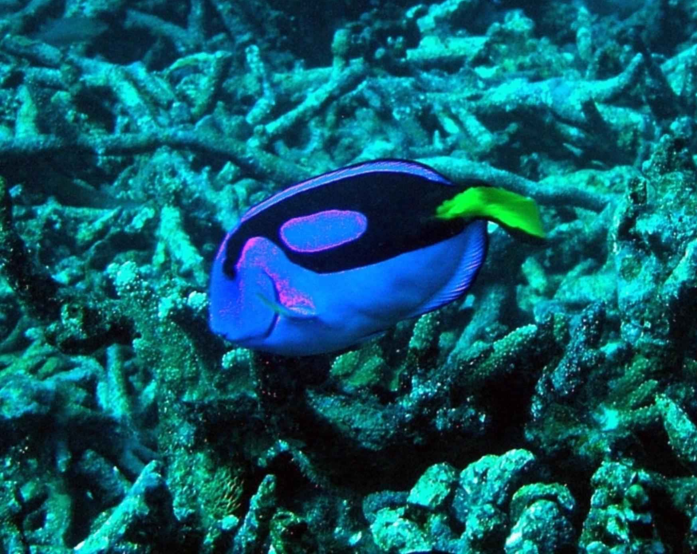
\includegraphics[width=3.8cm]{figures/dino_stage/ref_original_clean.png}
};
\node[imglbl] at (img_input.south) {1750 $\times$ 1392};
\draw[dashed, gray] (input.south) -- (img_input.north);

\node[below=2.0cm of resize, anchor=north] (img_resize) {
    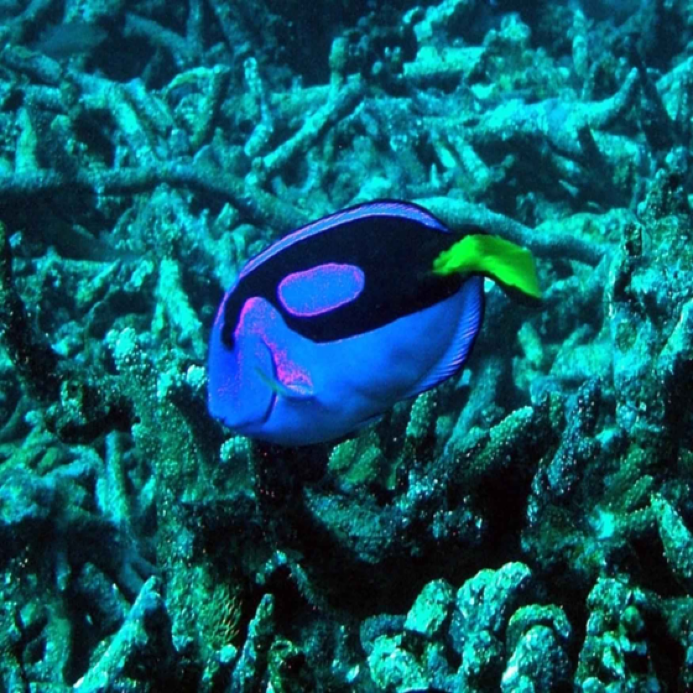
\includegraphics[width=3.8cm]{figures/dino_stage/ref_resized_clean.png}
};
\node[imglbl] at (img_resize.south) {560 $\times$ 560};
\draw[dashed, gray] (resize.south) -- (img_resize.north);

\node[below=2.0cm of dino, anchor=north] (img_dino) {
    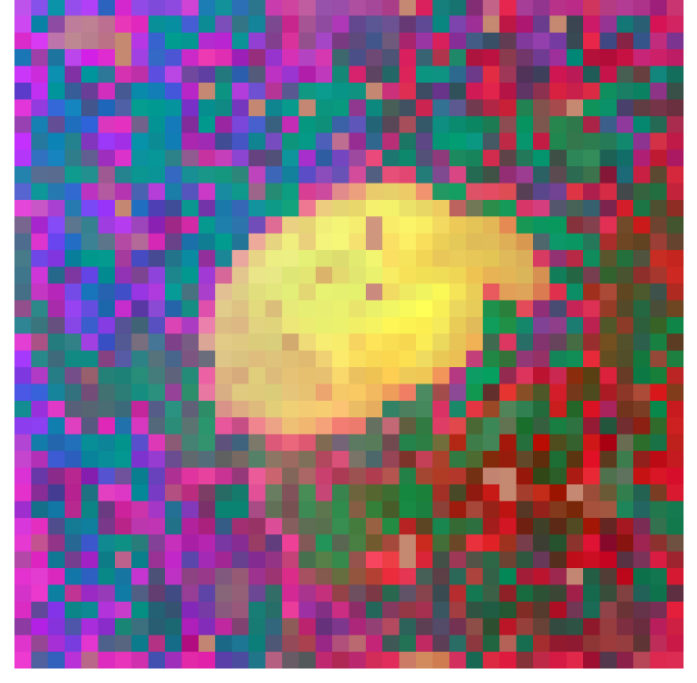
\includegraphics[width=3.8cm]{figures/dino_stage/ref_pca_features_clean.png}
};
\node[imglbl] at (img_dino.south) {1600 $\times$ 1536 (PCA)};
\draw[dashed, gray] (dino.south) -- (img_dino.north);

\node[below=2.0cm of features, anchor=north] (img_features) {
    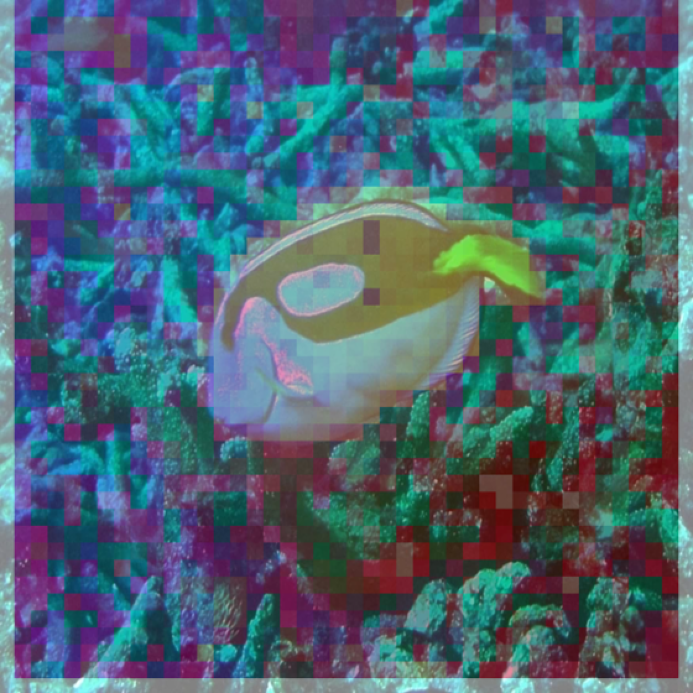
\includegraphics[width=3.8cm]{figures/dino_stage/ref_pca_features_overlay_clean.png}
};
\node[imglbl] at (img_features.south) {Features overlaid};
\draw[dashed, gray] (features.south) -- (img_features.north);


% Initial prompts image
\node[below=2.0cm of prompts, anchor=north] (img_prompts) {
    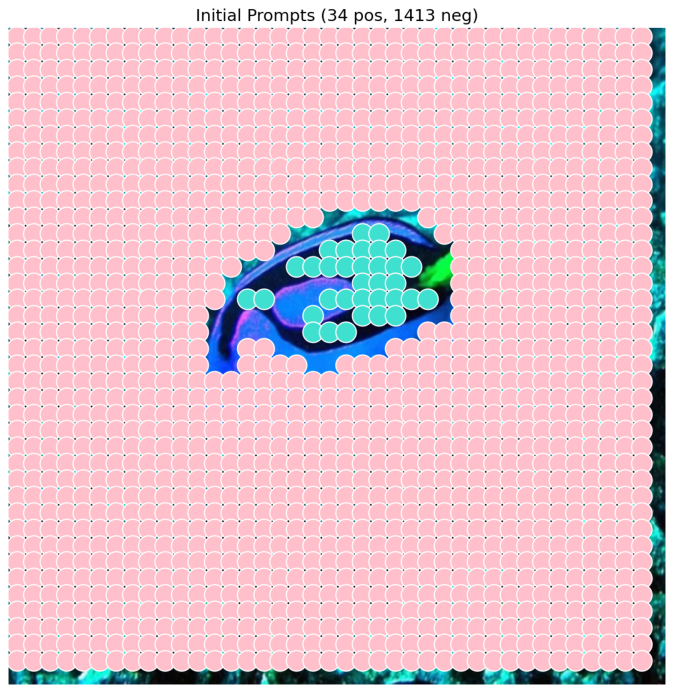
\includegraphics[width=3.8cm]{figures/dino_stage/prompts_clean.png}
};
\node[imglbl] at (img_prompts.south) {Pos/neg on target};
\draw[dashed, gray] (prompts.south) -- (img_prompts.north);

\end{tikzpicture}
\end{document}
